% Adjust these for the path of the theme and its graphics, relative to this file
%\usepackage{beamerthemeFalmouthGamesAcademy}
\usepackage{../../beamerthemeFalmouthGamesAcademy}
\usepackage{multimedia}
\graphicspath{ {../../} }

% Default language for code listings
\lstset{language=C++,
        morekeywords={each,in,nullptr,int32, TCHAR, uint8, int8, uint16, int16,
        uint32, int32, uint64, int64, PTRINT, UObject. AActor, SWidget, FName,
        FString, UClass, USoundCue, UTexture}
}

% For strikethrough effect
\usepackage[normalem]{ulem}
\usepackage{wasysym}
\usepackage{listings}
\usepackage{pdfpages}

% http://www.texample.net/tikz/examples/state-machine/
\usetikzlibrary{arrows,automata}

\newcommand{\modulecode}{COMP260}\newcommand{\moduletitle}{Distributed Systems}\newcommand{\sessionnumber}{5}

\begin{document}
\title{\sessionnumber: Inheritance and Polymorphism}
\subtitle{\modulecode: \moduletitle}

\frame{\titlepage}

\begin{frame}{Learning outcomes}
	\begin{itemize}
		\item \textbf{Understand} Inheritance in Object Orientated Programming
		\item \textbf{Understand} Polymorphism role in creating Games
		\item \textbf{Apply} your knowledge of Inheritance and Polymorphism to programming problems
	\end{itemize}
\end{frame}

\part{Object-oriented programming in C++}
\frame{\partpage}

\begin{frame}[fragile]{OOP refresher}
    \begin{itemize}
        \item A \textbf{class} is a collection of \textbf{fields} (data) and \textbf{methods} (functions)
        \item Fields and methods may be \textbf{public} (accessible everywhere), \textbf{protected} (accessible in the class and classes that inherit from it) or \textbf{private} (accessible in the class only)
        \item Classes may \textbf{inherit} fields and methods from other classes
        \item Subclasses may \textbf{override} methods which they inherit --- this gives rise to \textbf{polymorphism}
    \end{itemize}
\end{frame}

\begin{frame}[fragile]{Class declarations}
    \begin{lstlisting}
class MyClass
{
public:
    void doMethod(int x)
    {
        std::cout << x << std::endl;
    }

private:
    int field = 7;
};
    \end{lstlisting}
\end{frame}

\begin{frame}[fragile]{Fields and methods}
    \begin{itemize}
        \item Fields and methods are declared in the class declaration, just like variables and functions
        \item Class declaration is split into sections by access type (\textbf{public}, \textbf{protected}, \textbf{private})
    \end{itemize}
\end{frame}

\begin{frame}[fragile]{Overloading}
    \begin{itemize}
        \item Functions and methods can be defined with the \textbf{same name} but \textbf{different parameters}
    \end{itemize}
    \begin{lstlisting}
    double getVectorLength(double x, double y)
    {
        return sqrt(x * x + y * y);
    }

    double getVectorLength(Vector v)
    {
        return sqrt(v.x * v.x + v.y * v.y);
    }
    \end{lstlisting}
\end{frame}

\begin{frame}[fragile]{Constructors and destructors}
    \begin{itemize}
        \item The \textbf{constructor} is executed when the class is instantiated
        \item The \textbf{destructor} is executed when the instance is freed
    \end{itemize}
	\begin{lstlisting}
class MyClass
{
public:
    MyClass()
    {
    }
    
    ~MyClass()
    {
    }
};
	\end{lstlisting}
\end{frame}

\begin{frame}[fragile]{Constructors}
    \begin{itemize}
        \item The constructor name matches the class name
        \item Constructors can take parameters
        \item The constructor can be overloaded, i.e.\ can have several constructors with different parameters
    \end{itemize}
	\begin{lstlisting}
class MyClass
{
public:
    // Parameterless constructor
    MyClass() { }
    
    // Constructor with parameters
    MyClass(int x, double y) { }
};
	\end{lstlisting}
\end{frame}

\begin{frame}[fragile]{Destructors}
    \begin{itemize}
        \item The destructor name is the class name prefixed with $\sim$ (tilde)
        \item Destructors \textbf{cannot} take parameters
    \end{itemize}
\end{frame}

\begin{frame}[fragile]{Modular program design}
    \begin{itemize}
        \item Method \textbf{declarations} go in the class declaration
        \item Method \textbf{definitions} look like function definitions,
            with the function name replaced with \lstinline{ClassName::methodName}
        \item Method definitions can also go inline into the class declaration
        \begin{itemize}
            \item Best used for short (1 or 2 line) methods
        \end{itemize}
        \item Good practice: Put class declaration in \texttt{ClassName.h}, and method definitions in \texttt{ClassName.cpp}
    \end{itemize}
\end{frame}

\begin{frame}[fragile]{Example: Circle.h}
    \begin{lstlisting}
#pragma once

class Circle
{
public:
    Circle(double radius);
    
    double getArea();

private:
    double radius;
};
    \end{lstlisting}
\end{frame}

\begin{frame}[fragile]{Example: Circle.cpp}
    \begin{lstlisting}
#include "stdafx.h"
#include "Circle.h"

Circle::Circle(double radius)
    : radius(radius)
{
}

double Circle::getArea()
{
    return M_PI * radius * radius;
}
    \end{lstlisting}
\end{frame}

\begin{frame}[fragile]{Inheritance}
    \begin{lstlisting}
class Shape
{
public:
    virtual double getArea();
};

class Circle : Shape
{
public:
    virtual double getArea()
    {
        return M_PI * radius * radius;
    }
};
    \end{lstlisting}
    \begin{itemize}
        \item Methods to be overridden must be marked \textbf{virtual}
    \end{itemize}
\end{frame}

\begin{frame}[fragile]{Pure virtual methods}
    \begin{itemize}
        \item \textbf{Abstract classes} should never be instantiated --- they only exist to serve as a base class
        \item \textbf{Abstract methods} are not defined in the base class, and must be overridden in the subclass
        \item In C++, abstract methods are called \textbf{pure virtual}
        \item Having at least one pure virtual method \textbf{automatically} makes the class abstract
    \end{itemize}
    \begin{lstlisting}
class Shape
{
public:
    virtual double getArea() = 0;
};
    \end{lstlisting}
\end{frame}

\begin{frame}[fragile]{Instantiation}
    \begin{itemize}
        \item To instantiate with a \textbf{parameterless constructor}, just declare a variable
    \end{itemize}
    \begin{lstlisting}
MyClass myInstance;
    \end{lstlisting}
    \begin{itemize}
        \item To instantiate with a \textbf{constructor with parameters}, add the parameters in parentheses
    \end{itemize}
    \begin{lstlisting}
MyClass myInstance(27);
    \end{lstlisting}
    \begin{itemize}
        \item This allocates the instance on the \textbf{stack}
        \item The instance is destroyed (and the destructor is called) when the variable goes \textbf{out of scope}
    \end{itemize}
\end{frame}


\part{Inheritance}
\frame{\partpage}

\begin{frame}{Introduce to Inheritance}
	\begin{itemize}
		\pause \item One of the key features of OOP languages is \textbf{Inheritance}
		\pause \item This allows you to \textbf{Derive} a new class from an existing one
		\pause \item When this is done, the new class automatically inherits the variables and functions of the \textbf{parent} class
		\pause \item Advantages of inheritance includes
		\begin{itemize}
			\pause \item Code reuse: There is no need to redefine functionality, you can just inherit from a base class
			\pause \item Fewer errors: If you build on existing class that is bug free then you are more likely to have less errors
			\pause \item Cleaner code: because of the increase of code reuse then your code is more modular and reusable. 
		\end{itemize}
	\end{itemize}
\end{frame}

\begin{frame}[fragile]{Inheritance Example - C\#}
		\begin{lstlisting}[language=C++,basicstyle=\tiny,]
		public class Enemy : MonoBehaviour
		{
			[SerializeField]
			proteced int Damage;
			
			void Start()
			{
				Damage=1;
			}
			
			public void Attack()
			{
				Debug.Log("The attack causes "+Damage.ToString()+" damage");
			}
		}
		\end{lstlisting}
\end{frame}

\begin{frame}[fragile]{Inheritance Example - C\#}
	\begin{lstlisting}[language=C++,basicstyle=\tiny,]
	public class Boss : Enemy
	{
		[SerializeField]
		private int DamageMultiplier; 
		
		void Start()
		{
			Damage=5;
			DamageMultipler=2;
		}
		
		public void Attack()
		{
			Debug.Log("The attack causes "+Damage.ToString()+" damage");
		}
		
		public void SpecialAttack()
		{
			int totalDamage=Damage*DamageMultiplier;
			Debug.Log("Special attack causes "+totalDamage.ToString()+" damage");
		}
	}
	\end{lstlisting}
\end{frame}

\begin{frame}[fragile]{Inheritance Example - C++}
	\begin{lstlisting}[language=C++,basicstyle=\tiny,]
	public class Enemy
	{
		public:
			Enemy()
			{
				Damage=1;
			};
			
			virtual ~Enemy()
			{
			}
			
			void Attack()
			{
				std::cout<<"The attack causes "<<Damage<<" damage"<<std::endl;
			}
		protected:
			int Damage;
	}
	\end{lstlisting}
\end{frame}

\begin{frame}[fragile]{Inheritance Example - C++}
	\begin{lstlisting}[language=C++,basicstyle=\tiny,]
	public class Boss : public Enemy
	{
		public:
			Boss()
			{
				Damage=5;
				DamageMultiplier=2;
			};
			
			~Boss()
			{
			}
			
			void SpecialAttack()
			{
				int totalDamage=Damage*DamageMultiplier;
				std::cout<<"Special attack causes "<<totalDamage<<" damage"<<std::endl;
			}	
		protected:
			int DamageMultiplier;
		

	}
	\end{lstlisting}
\end{frame}

\begin{frame}{Overriding}
	\begin{itemize}
		\pause \item You can override functions in the base class by providing a new version of the function
		\pause \item You should mark any function that you are going to override with the \textbf{virtual} keyword 
		\pause \item Then in the child class, you have a function with the same signature which is marked with the \textbf{override} keyword
	\end{itemize}
\end{frame}

\begin{frame}[fragile]{Overriding Example - C\#}
	\begin{lstlisting}[language=C++,basicstyle=\tiny,]
		public class Enemy : MonoBehaviour
		{
			[SerializeField]
			proteced int Damage;
		
			void Start()
			{
				Damage=1;
			}
		
			public virtual void Attack()
			{
				Debug.Log("The attack causes "+Damage.ToString()+" damage");
			}
		}
	\end{lstlisting}
\end{frame}

\begin{frame}[fragile]{Overriding Example - C\#}
	\begin{lstlisting}[language=C++,basicstyle=\tiny,]
		public class Boss : Enemy
		{
		
		void Start()
		{
			Damage=5;
		}
		
		public override void Attack()
		{
			base.Attack();
			Damage+=1;
			Debug.Log("This is the boss attacking");
		}
		
	\end{lstlisting}
\end{frame}

\begin{frame}[fragile]{Overriding Example - C++}
	\begin{lstlisting}[language=C++,basicstyle=\tiny,]
	public class Enemy
	{
	public:
		Enemy()
		{
			Damage=1;
		};
		
		virtual ~Enemy()
		{
		}
	
		virtual void Attack()
		{
			std::cout<<"The attack causes "<<Damage<<" damage"<<std::endl;
		}
	protected:
		int Damage;
	}
	\end{lstlisting}
\end{frame}

\begin{frame}[fragile]{Overriding Example - C++}
	\begin{lstlisting}[language=C++,basicstyle=\tiny,]
	public class Boss : public Enemy
	{
	public:
		Boss()
		{
			Damage=5;
		};
	
		~Boss()
		{
		}
	
		void Attack() override
		{
			Enemy::Attack();
			Damage+=1;
			std::cout<<"This is the boss attacking"<<std::endl;
		}	
	protected:
		int DamageMultiplier;
	}
	\end{lstlisting}
\end{frame}

\begin{frame}{Abstract Classes \& Interfaces}
\end{frame}

\part{Polymorphism}
\frame{\partpage}

\begin{frame}{Polymorphism}
\begin{itemize}
	\pause\item From Greek: ``many-shape-ism''
	\pause\item Different classes can have the \textbf{same public interface}
	\pause\item Thus we can write code that \textbf{uses} this interface, but doesn't need to worry about the \textbf{implementation} behind it
\end{itemize}
\end{frame}

\begin{frame}{Method overriding}
\begin{itemize}
	\pause\item A class can \textbf{override} methods defined in the class from which it inherits
	\pause\item The overridden method can call the method from the base class, but it doesn't have to
\end{itemize}
\end{frame}

\begin{frame}[fragile]{Without polymorphism}
	\begin{lstlisting}
class Shape { ... };
class Circle : public Shape { ... };
class Square : public Shape { ... };
class Triangle : public Shape { ... };

std::vector<Shape*> shapes;
// Populate shapes with circles, squares, triangles...

for (Shape* shape : shapes)
{
	if (shape->isCircle)
		drawCircle(shape->centre, shape->radius);
	else if (shape->isSquare)
		drawSquare(shape->centre, shape->size);
	...
}
	\end{lstlisting}
\end{frame}

\begin{frame}[fragile]{Polymorphism to the rescue!}
	\begin{lstlisting}
class Shape {
	public: virtual void draw() {}
};
class Circle : public Shape {
	public: void draw() override {
		drawCircle(centre, radius);
	}
};
class Square : public Shape {
	public: void draw() override {
		drawSquare(centre, size);
	}
};

for (Shape* shape : shapes)
	shape->draw();
	\end{lstlisting}
\end{frame}

\begin{frame}{Polymorphism to the rescue!}
	\begin{itemize}
		\pause\item All subclasses of \lstinline{Shape} implement \lstinline{draw}
		\pause\item We can call \lstinline{shape->draw()} without worrying which type of shape it is
		\pause\item The \textbf{virtual method table} takes care of calling the correct
			\lstinline{draw} function depending on the type of \lstinline{shape},
			no extra code required
	\end{itemize}
\end{frame}

\begin{frame}[fragile]{Instance types}
	\pause
	\begin{lstlisting}
Shape myShape;
	\end{lstlisting}
	\begin{itemize}
		\pause\item \lstinline{myShape} is an instance of \lstinline{Shape}, allocated on the \textbf{stack}
	\end{itemize}
	\pause
	\begin{lstlisting}
Shape* myShapePtr;
	\end{lstlisting}
	\begin{itemize}
		\pause\item \lstinline{myShapePtr} points to an instance of \lstinline{Shape}
			or of a subclass of \lstinline{Shape}, allocated on the \textbf{heap}
		\pause\item Polymorphism works for pointers, but not for instances on the stack
	\end{itemize}
\end{frame}

\begin{frame}{Abstract classes}
\begin{itemize}
	\pause\item Some classes should never be instantiated directly, as they only exist to be inherited from
	\begin{itemize}
		\pause\item \lstinline{Shape} is an example
	\end{itemize}
	\pause\item Such classes are called \textbf{abstract}
	\pause\item Abstract classes generally have one or more \textbf{pure virtual methods} ---
		methods which are left unimplemented so \textbf{must} be implemented in subclasses
\end{itemize}
\end{frame}

\begin{frame}[fragile]{Abstract class example}
	\begin{lstlisting}
class Shape
{
public:
	virtual void draw() = 0;
};
	\end{lstlisting}
	\begin{itemize}
		\pause\item Here \lstinline{= 0} marks the method as \textbf{pure virtual}
		\pause\item In C++, having at least one pure virtual method implicitly marks the class as \textbf{abstract}
		\pause\item Now you will get a compile error if you try to instantiate \lstinline{Shape} directly
		\pause\item To become not abstract, subclasses of \lstinline{Shape} must override \lstinline{draw}
		\pause\item Subclasses of \lstinline{Shape} which \textbf{do} override \lstinline{draw} can be instantiated
		\pause\item Trying to instantiate a subclass of \lstinline{Shape} which \textbf{does not} override \lstinline{draw}
			will also give a compile error
	\end{itemize}
\end{frame}

\begin{frame}[fragile]{Interfaces}
	\begin{itemize}
		\pause\item An abstract class in which \textbf{all} methods are pure virtual is called an \textbf{interface}
		\pause\item Interfaces do not contain any implementation, but specify a set of methods which subclasses
			must implement
		\pause\item NB: some languages (e.g.\ C\#, Java) make a distinction between classes and interfaces;
			C++ does not
	\end{itemize}
\end{frame}

\begin{frame}{OOP design}
	\begin{center}
		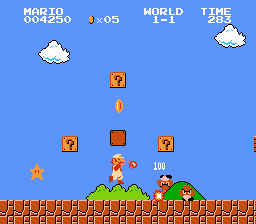
\includegraphics[height=0.4\textheight]{mario}
		\hspace{0.1\textwidth}
		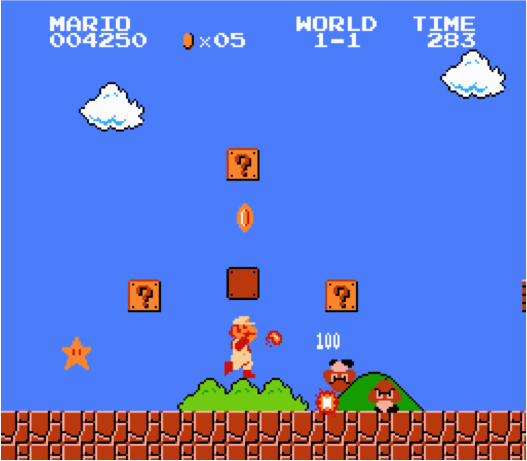
\includegraphics[height=0.4\textheight]{mario2}
	\end{center}
	\begin{itemize}
		\item What \textbf{classes} might be defined in a Mario-style platform game?
		\item What classes might \textbf{inherit} from one another?
	\end{itemize}
\end{frame}

\part{Coffee Break}
\frame{\partpage}
\part{Exercises}
\frame{\partpage}

\begin{frame}{Exercise 1 - Texturing}
	\begin{itemize}
		\item Load in a image using SDL Image
		\item Copy this image into a OpenGL Texture
		\item Add Texture Coordinates to your Cube or Square
		\item Map this texture onto the Cube or Square
		\item Finally change the texture to a transparent texture
	\end{itemize}
\end{frame}

\begin{frame}{Exercise 2 - Model Loading}
	\begin{itemize}
		\item Create the following NFF models and load each one to the screen
		\begin{itemize}
			\item Tetrahedron 
			\item Cube
			\item Sphere
			\item Cylinder
		\end{itemize}
		\item \url{http://assimp.sourceforge.net/howtoBasicShapes.html}
		\item \url{https://github.com/assimp/assimp/tree/master/test/models/NFF/NFF}
	\end{itemize}
\end{frame}

\begin{frame}{Exercise 3 - More Complex Scene}
	\begin{itemize}
		\item Create a GameObject class which contains the following as member variables
		\begin{itemize}
			\item Vertex Buffer
			\item Element Buffer
			\item Vertex Array Object
			\item Position, Scale, Rotation Vectors
			\item Position, Scale, Rotation, Model Matrices
			\item Open GL Texture
			\item Number of vertices and Indices
		\end{itemize}
		\item Add in functions to initialise and get each of these values
		\item Add in functions to update (calculate the model matrix) and render
		\item Create an instance of this Game Object and display it on the screen
	\end{itemize}
\end{frame}

\begin{frame}{References}
	\begin{itemize}
		\item Dawson, M. Beginning C++ through game programming 4th Ed. Chapter 8 - 10 \url{http://voyager.falmouth.ac.uk/vwebv/holdingsInfo?bibId=1097178}
		\item \url{https://www.geeksforgeeks.org/inheritance-in-c/}
		\item \url{https://www.geeksforgeeks.org/pure-virtual-functions-and-abstract-classes/}
	\end{itemize}
\end{frame}


\end{document}
